\documentclass[aspectratio=169,professionalfonts]{beamer}

\usetheme{metropolis}
\setbeamertemplate{navigation symbols}{}
\setbeamertemplate{footline}[frame number]

\usepackage{fontspec}
\setsansfont{Fira Sans}

\usepackage{amsmath}
\usepackage{graphicx}
\usepackage{booktabs}
\usepackage{xcolor}

% Professional dark-navy / steel-blue palette
\definecolor{Primary}{HTML}{1B2A4A}   % dark navy
\definecolor{Accent}{HTML}{2D7DD2}    % steel blue
\definecolor{Alert}{HTML}{E76F51}     % burnt orange

\setbeamercolor{frametitle}{bg=Primary}
\setbeamercolor{progress bar}{fg=Accent}
\setbeamercolor{alerted text}{fg=Alert}

\title{StreamCab}
\subtitle{Real-Time Taxi Fare Intelligence\\Kafka · Spark Structured Streaming · XGBoost}
\author{ Bibek Dhungana, Xiaodi Shao, Raivath Mallela}
\institute{Data Engineering}
\date{\today}

\begin{document}

\maketitle

% Agenda 
\begin{frame}{Agenda (12 min + 3 min Q\&A)}
\begin{enumerate}
  \item \textbf{Overview} — problem statement and system architecture
  \item \textbf{Data} — source, collection, schema, and metadata
  \item \textbf{Process} — end-to-end pipeline inputs and outputs
  \item \textbf{Results} — dashboard, model quality, and insights
  \item \textbf{Takeaways} — what worked and what was hard
\end{enumerate}
\end{frame}

%
\section{Overview}

\begin{frame}{Problem Statement}
\Large
NYC taxi demand and pricing shift rapidly by zone and time.

\vspace{0.8em}
\normalsize
\begin{itemize}
  \item Static batch reports lag behind operational decisions.
  \item No live view of which zones are surging right now.
  \item Fare prediction from historical patterns alone is too slow.
\end{itemize}

\vspace{0.8em}
\alert{Goal:} Build a full streaming analytics and prediction stack — ingestion
to live dashboard — that runs reproducibly on a single machine.
\end{frame}

\begin{frame}{System Architecture}
\centering
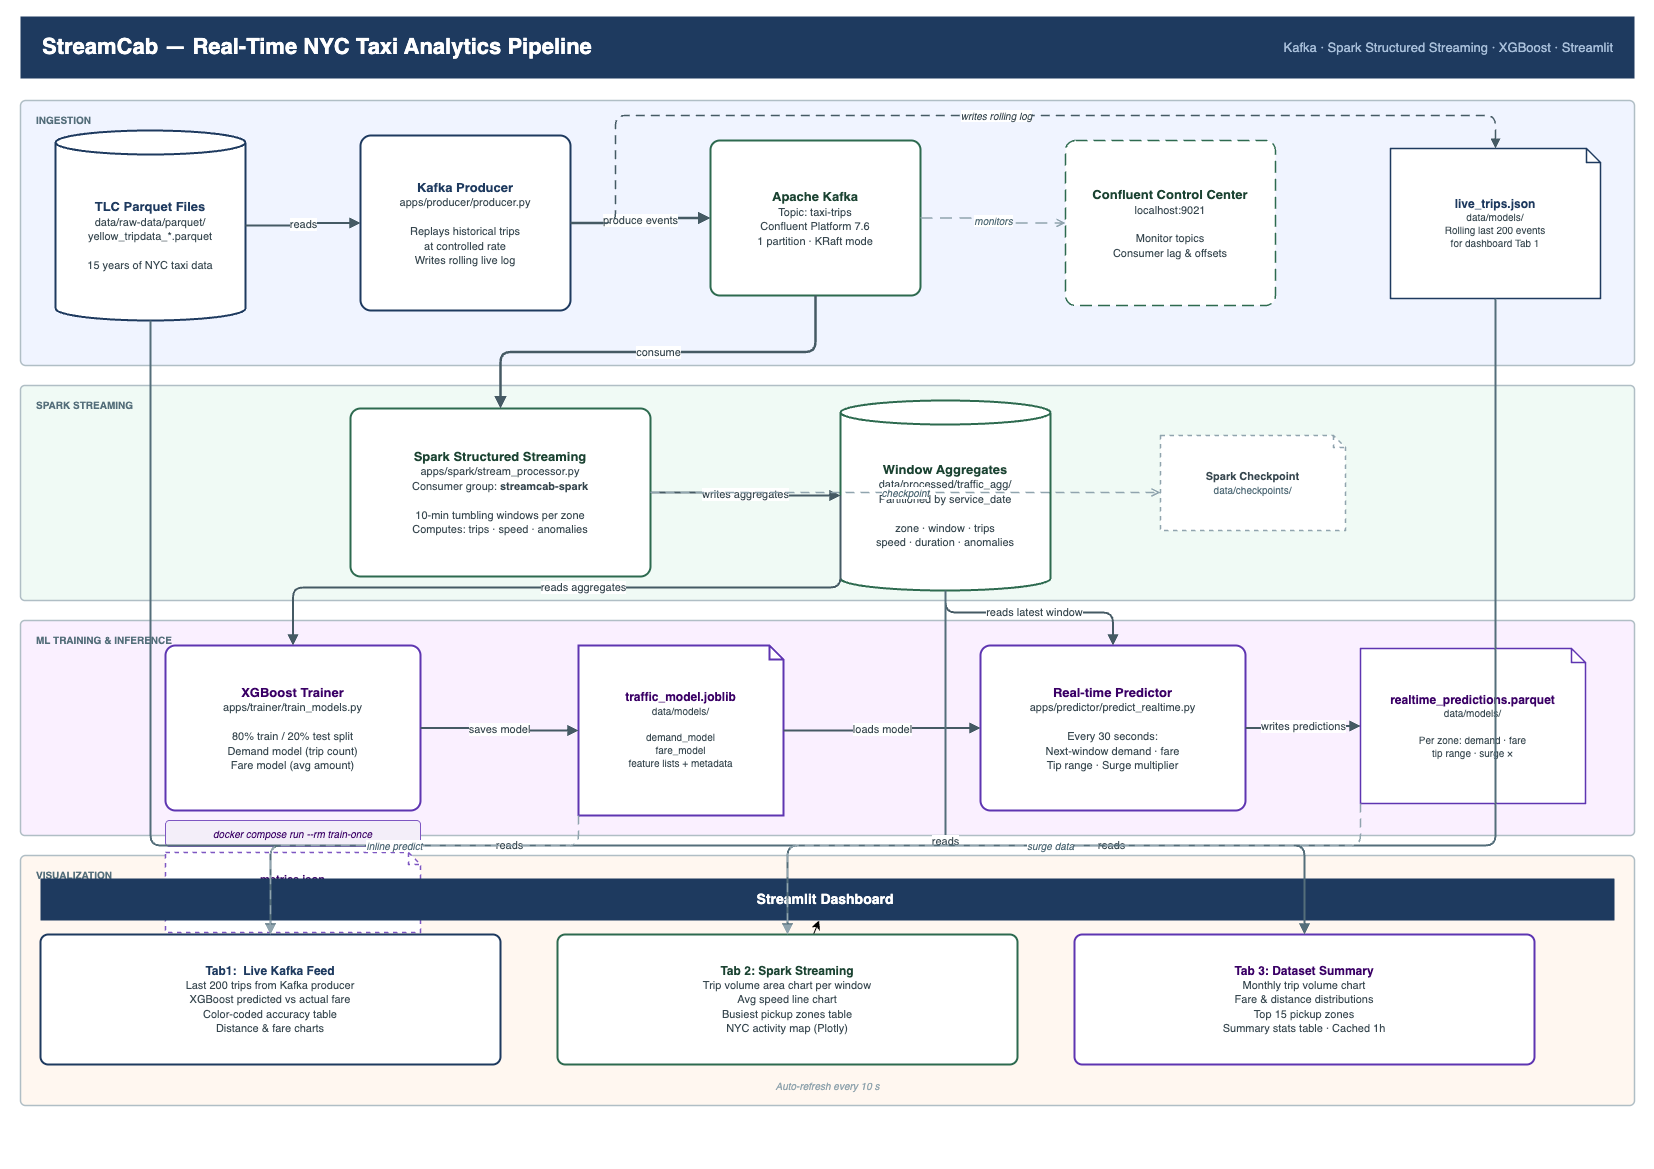
\includegraphics[width=0.90\textwidth,height=0.72\textheight,keepaspectratio]{../assets/architecture.png}

\vspace{0.2em}
\small Parquet $\to$ Kafka $\to$ Spark $\to$ PostgreSQL $\to$ Predictor $\to$ Dashboard
\end{frame}

\begin{frame}{Architecture Components}
\begin{columns}[T]
\column{0.5\textwidth}
\begin{itemize}
  \item \textbf{Producer + Kafka:} replay trips as a live event stream
  \item \textbf{Consumer:} write raw events to \texttt{live\_trips}
  \item \textbf{Spark:} 10-min windowed zone aggregates
  \item \textbf{PostgreSQL:} live trips, aggregates, predictions
\end{itemize}

\column{0.5\textwidth}
\begin{itemize}
  \item \textbf{Trainer:} XGBoost on historical aggregates
  \item \textbf{Predictor:} periodic inference every 30 s
  \item \textbf{Dashboard:} live KPIs, map, zone rankings
\end{itemize}
\vspace{0.5em}
\textbf{Tools not in class:} Kafka (pub/sub event log),
Spark Structured Streaming (stateful DataFrames),
psycopg (Python--PostgreSQL bridge)
\end{columns}
\end{frame}

%
\section{Data}

\begin{frame}{Data Source and Collection}
\textbf{Source:} NYC TLC Yellow Taxi Trip Records — public monthly Parquet files\\
\small\texttt{nyc.gov/site/tlc/about/tlc-trip-record-data.page}\normalsize

\vspace{0.5em}
\textbf{Collection workflow}
\begin{enumerate}
  \item Download monthly parquet files via project script (retry + back-off).
  \item Store under \texttt{/data/raw-data/parquet/}.
  \item Producer replays rows to Kafka as pseudo-live events.
\end{enumerate}

\vspace{0.5em}
\textbf{Scale:} 2015--2025 supported; default pull 2022-01 → 2024-12;
quick-start uses 2022-01 → 2022-03 for fast local iteration.\\[0.4em]
\textbf{Reference data:} TLC zone centroid CSV for spatial zone mapping.
\end{frame}

\begin{frame}{Schema and Metadata}
\begin{columns}[T]
\column{0.5\textwidth}
\textbf{Raw event fields}
\begin{itemize}
  \item \texttt{pickup\_datetime}, \texttt{dropoff\_datetime}
  \item \texttt{passenger\_count}, \texttt{trip\_distance}
  \item \texttt{pu\_location\_id}, \texttt{do\_location\_id}
  \item \texttt{total\_amount}, \texttt{emitted\_at}
\end{itemize}

\column{0.5\textwidth}
\textbf{Windowed aggregate fields}
\begin{itemize}
  \item \texttt{window\_start}, \texttt{window\_end}
  \item \texttt{pu\_location\_id}, \texttt{trip\_count}
  \item \texttt{avg\_trip\_distance}, \texttt{avg\_duration\_min}
  \item \texttt{avg\_speed\_mph}, \texttt{avg\_total\_amount}
  \item \texttt{anomaly\_count}
\end{itemize}
\end{columns}

\vspace{0.6em}
Pre-2017 files (lat/lon format) are snapped to nearest zone centroid via
BallTree ($\approx$100 m precision).
\end{frame}

\begin{frame}{Data Quality Rules}
Rows are retained only when they satisfy all bounds:

\vspace{0.4em}
\begin{center}
\begin{tabular}{ll}
\toprule
Field & Accepted range \\
\midrule
Duration & 1--180 min \\
Trip distance & 0.2--100 mi \\
Average speed & 1--80 mph \\
Fare / total amount & \$0--\$500 \\
Pickup zone & valid ID or mappable lat/lon \\
\bottomrule
\end{tabular}
\end{center}

\vspace{0.4em}
Conservative filtering reduces outlier influence and improves model stability.
\end{frame}

%
\section{Process}

\begin{frame}{End-to-End Processing Pipeline}
\begin{enumerate}
  \item \textbf{Ingest} — read parquet, normalize timestamps and zone IDs.
  \item \textbf{Stream} — replay rows to Kafka at configurable rate.
  \item \textbf{Aggregate} — Spark applies quality filters; computes 10-min window stats per zone.
  \item \textbf{Persist} — consumer writes \texttt{live\_trips}; Spark upserts \texttt{traffic\_agg}.
  \item \textbf{Train} — XGBoost reads aggregates in memory-aware batches.
  \item \textbf{Predict} — predictor scores latest windows every 30 s.
  \item \textbf{Visualize} — Streamlit renders KPIs, zone rankings, and map.
\end{enumerate}
\end{frame}

\begin{frame}{Inputs and Outputs}
\begin{columns}[T]
\column{0.33\textwidth}
\textbf{Inputs}
\begin{itemize}
  \item Historical Parquet trip files
  \item Zone centroid CSV
\end{itemize}

\column{0.33\textwidth}
\textbf{Intermediates}
\begin{itemize}
  \item Kafka topic \texttt{taxi-trips}
  \item \texttt{live\_trips} table
  \item \texttt{traffic\_agg} table
  \item Spark checkpoints
\end{itemize}

\column{0.33\textwidth}
\textbf{Final outputs}
\begin{itemize}
  \item \texttt{traffic\_model}\\\texttt{.joblib}
  \item \texttt{metrics.json}
  \item \texttt{predictions} table
  \item Live dashboard
\end{itemize}
\end{columns}
\end{frame}

\begin{frame}{Model Training Configuration}
\begin{columns}[T]
\column{0.5\textwidth}
\textbf{Target:} \texttt{avg\_total\_amount}

\vspace{0.4em}
\textbf{Features (8):}
\begin{itemize}\small
  \item \texttt{pu\_location\_id}, \texttt{hour}
  \item \texttt{day\_of\_week}, \texttt{is\_weekend}
  \item \texttt{avg\_trip\_distance}, \texttt{avg\_duration\_min}
  \item \texttt{avg\_speed\_mph}, \texttt{trip\_count}
\end{itemize}

\column{0.5\textwidth}
\textbf{XGBoost settings:}\small
\begin{itemize}
  \item \texttt{max\_depth=5}, \texttt{lr=0.05}
  \item \texttt{subsample=0.9}, \texttt{tree\_method=hist}
  \item 80/20 temporal train-test split
\end{itemize}

\normalsize\vspace{0.4em}
\textbf{Strategy:} 500K-row parquet batches; continued boosting (+40 trees/batch);
best validation-MAE checkpoint selected.
\end{columns}
\end{frame}

% 
\section{Results}

\begin{frame}{Model Performance}
\Large
\begin{center}
\begin{tabular}{lcc}
\toprule
Model & MAE (\$) & MAPE (\%) \\
\midrule
Baseline (zone-hour mean) & 1.99 & 15.43 \\
\textbf{XGBoost (test)} & \textbf{0.49} & \textbf{3.42} \\
\bottomrule
\end{tabular}
\end{center}

\vspace{0.8em}
\normalsize
\alert{75\% reduction in MAE} over the baseline. XGBoost captures nonlinear
interactions between demand, speed, duration, and time that a simple mean
cannot represent.
\end{frame}

\begin{frame}{Dashboard and Analytics Outputs}
\centering
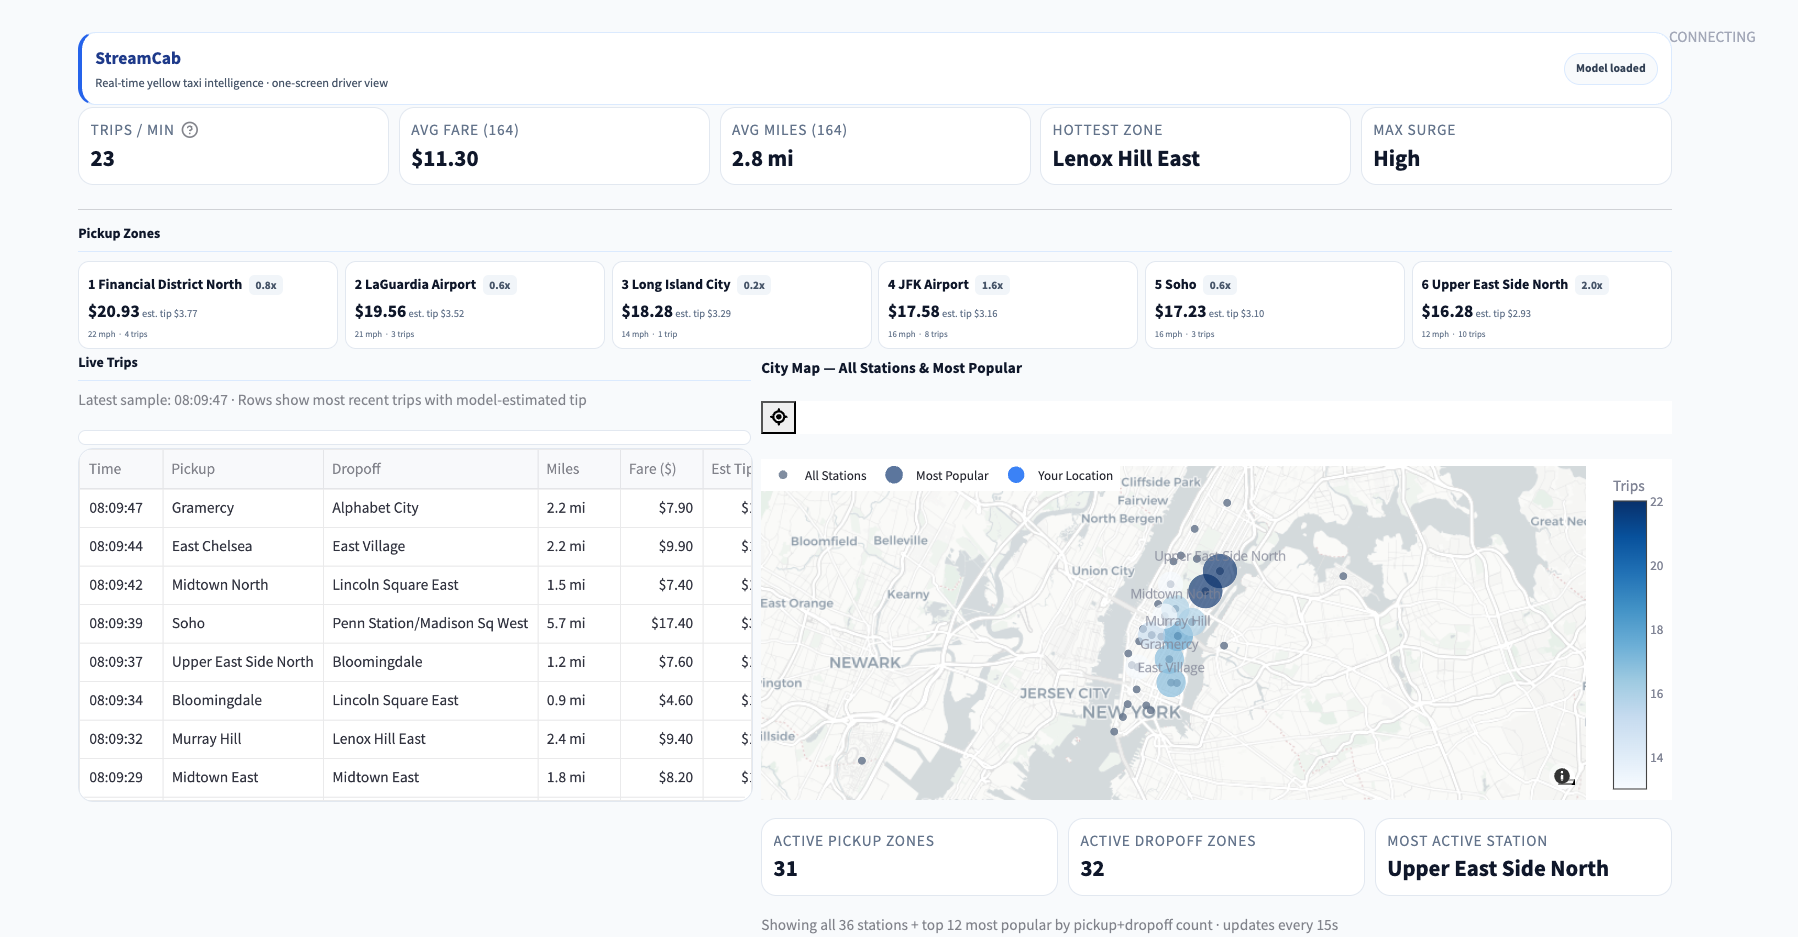
\includegraphics[width=0.88\textwidth,height=0.70\textheight,keepaspectratio]{../assets/app.png}

\vspace{0.2em}
\small Live KPIs · zone rankings with surge badges · NYC map · rolling trip table
\end{frame}

% 
\section{Key Takeaways}

\begin{frame}{What Worked and What Was Hard}
\begin{columns}[T]
\column{0.5\textwidth}
\textbf{Worked well}
\begin{itemize}
  \item Reproducible one-command startup with Docker Compose.
  \item Spark windowed aggregates as stable, interpretable features.
  \item Strong prediction accuracy with XGBoost.
  \item Memory-aware batch training on limited hardware.
\end{itemize}

\column{0.5\textwidth}
\textbf{Most difficult}
\begin{itemize}
  \item Training at scale under local memory constraints.
  \item Cross-service reliability between Kafka, Spark, and PostgreSQL.
  \item Pre-2017 TLC format changes (lat/lon vs.\ zone IDs).
  \item Spark checkpoint tuning for stable restarts.
\end{itemize}
\end{columns}

\vspace{0.6em}
\textbf{Future work:} drift monitoring, automated retraining, exogenous
signals (weather/events), quantile outputs, cloud-scale deployment.
\end{frame}

\begin{frame}{Submission Checklist}
\begin{itemize}
  \item[$\checkmark$] GitHub repo with README walkthrough (data input $\to$ final output)
  \item[$\checkmark$] Public data source: \texttt{nyc.gov/site/tlc/about/tlc-trip-record-data.page}
  \item[$\checkmark$] Final report in IEEE research paper style (6--8 pages)
  \item[$\checkmark$] Abstract, Introduction, Related Work, Architecture, Data, Results, Conclusion
  \item[$\checkmark$] Presentation covers all five required sections
  \item[$\checkmark$] Brief intro to tools not in class (Kafka, Spark Streaming, psycopg, XGBoost)
  \item[$\circ$] \alert{Add all group member names to report and presentation}
\end{itemize}
\end{frame}

\begin{frame}[standout]
Questions?

\vspace{0.5em}
\normalsize
\texttt{github.com/dhunganabibek/StreamCab}
\end{frame}

\end{document}
